% SOLVING LINEAR EQUATIONS IN ONE VARIABLE - WORKSHEET 0 (IN-CLASS INSTRUCTION)
\documentclass[12pt, letterpaper, fleqn]{article}

% ----------------------------------------------------------
% PACKAGES
% ----------------------------------------------------------
\usepackage{graphicx}
\usepackage{xcolor}
\usepackage[most]{tcolorbox}
\usepackage{amsmath, amssymb}
\usepackage{fancyhdr}
\usepackage[utf8]{inputenc}
\usepackage[T1]{fontenc}
\usepackage{enumitem}
\usepackage{geometry}
\usepackage{tikz}
\usepackage{needspace}
\usepackage{multicol}

\usetikzlibrary{arrows.meta, calc}

% ----------------------------------------------------------
% PAGE SETUP
% ----------------------------------------------------------
\usepackage{times}
\geometry{letterpaper, top=1.25in, bottom=1.25in, marginpar=0.5in}

% ----------------------------------------------------------
% HEADER / FOOTER
% ----------------------------------------------------------
\newcommand{\logowidth}{3cm}
\setlength{\headheight}{20pt}
\setlength{\footskip}{40pt}

\pagestyle{fancy}
\fancyhf{}
\fancyhead[C]{\small\bfseries Solving Linear Equations in One Variable}
\fancyfoot[L]{\raisebox{2pt}{
\includegraphics[width=\logowidth]{../kss.png}}}
\fancyfoot[C]{\thepage}
\fancyfoot[R]{8.10.0}

\renewcommand{\footrulewidth}{0.2pt}

% ----------------------------------------------------------
% THEME COLOR
% ----------------------------------------------------------
\definecolor{customteal}{HTML}{2fbdb9}

% ----------------------------------------------------------
% HELPER MACROS
% ----------------------------------------------------------
\newcommand{\blank}{\underline{\hspace{2.2cm}}}
\newcommand{\blanklong}{\underline{\hspace{6.5cm}}}
\newcommand{\blankshorter}{\underline{\hspace{1.5cm}}}

% ----------------------------------------------------------
% DOCUMENT
% ----------------------------------------------------------
\begin{document}

\textbf{Name:} \underline{\hspace{5cm}}
\hfill
\textbf{Date:} \underline{\hspace{3cm}}\\

% ==========================================================
% SECTION 1: FOUNDATION
% ==========================================================
\begin{tcolorbox}[colback=customteal!20]
    \large\textcolor{black}{\textbf{Foundation: Solving Linear Equations}}
\end{tcolorbox}

\vspace{3mm}

\noindent
Solving an equation means finding the value of the variable (like $x$) that makes the equation true. We do this by \textbf{isolating} the variable using inverse operations, keeping the equation balanced.

\begin{itemize}
    \item \textbf{Variables on Both Sides:} If $x$ is on both sides, add or subtract the $x$ terms to get them all on one side of the equal sign.
    \item \textbf{Distributive Property:} If you see parentheses, distribute first: $a(b + c) = ab + ac$.
    \item \textbf{Like Terms:} Combine terms that have the same variable on the same side of the equation before moving them across the equal sign.
\end{itemize}

\vspace{4mm}

% ==========================================================
% VISUAL REPRESENTATION
% ==========================================================
\begin{tcolorbox}[colback=white, colframe=black!25, boxrule=0.6pt, arc=4mm, left=6mm, right=6mm, top=5mm, bottom=5mm]

\textbf{Visual Representation: A Balanced Scale}

\medskip

\begin{center}
\begin{tikzpicture}[scale=0.8]

% Scale Base
\draw[thick] (-2, 0) -- (2, 0);
\draw[thick] (0, 0) -- (0, 3);
\draw[thick] (-3, 3) -- (3, 3);
\filldraw[black] (0, 3) circle (3pt);

% Left Side
\draw[thick] (-3, 3) -- (-3, 2);
\draw[thick] (-4, 2) -- (-2, 2);
% Left items (2x + 4)
\filldraw[fill=blue!30, draw=blue, thick] (-3.5, 2) rectangle (-2.5, 3);
\node at (-3, 2.5) {$x$};
\filldraw[fill=blue!30, draw=blue, thick] (-3.5, 3) rectangle (-2.5, 4);
\node at (-3, 3.5) {$x$};
\draw[fill=green!30, draw=green!50!black, thick] (-2.3, 2) circle (0.3); \node at (-2.3, 2) {$4$};

% Right Side
\draw[thick] (3, 3) -- (3, 2);
\draw[thick] (2, 2) -- (4, 2);
% Right items (x + 10)
\filldraw[fill=blue!30, draw=blue, thick] (2.5, 2) rectangle (3.5, 3);
\node at (3, 2.5) {$x$};
\draw[fill=green!30, draw=green!50!black, thick] (3.8, 2) circle (0.4); \node at (3.8, 2) {$10$};

\end{tikzpicture}
\end{center}

\medskip
\begin{itemize}
    \item The scale shows $2x + 4 = x + 10$.
    \item If we remove one $x$-box from both sides, the scale stays balanced: $x + 4 = 10$.
    \item If we remove $4$ from both sides, we get $x = 6$.
\end{itemize}

\end{tcolorbox}

\vspace{4mm}

\newpage

% ==========================================================
% WORKED EXAMPLES
% ==========================================================
\begin{tcolorbox}[colback=customteal!20]
\large\textcolor{black}{\textbf{Solving Step-by-Step}}
\end{tcolorbox}

\noindent
Follow the order: 1) Distribute, 2) Combine like terms, 3) Variables to one side, 4) Isolate variable.

\vspace{3mm}

\begin{tcolorbox}[colback=white, colframe=black!25, boxrule=0.6pt, arc=4mm, left=6mm, right=6mm, top=5mm, bottom=5mm]

\textbf{Worked Example 1: Variables on Both Sides with Distribution}

\medskip

\textbf{Problem:} Solve $3(2x - 4) = 4x + 10$.

\medskip

\textbf{Solution:}
\begin{itemize}
    \item \textbf{Step 1 (Distribute):} Multiply $3$ by $(2x)$ and $3$ by $(-4)$.
    \begin{align*}
        6x - 12 &= 4x + 10
    \end{align*}
    \item \textbf{Step 2 (Variables to one side):} Subtract $4x$ from both sides.
    \begin{align*}
        6x - 4x - 12 &= 10 \\
        2x - 12 &= 10
    \end{align*}
    \item \textbf{Step 3 (Isolate variable term):} Add $12$ to both sides.
    \begin{align*}
        2x &= 10 + 12 \\
        2x &= 22
    \end{align*}
    \item \textbf{Step 4 (Divide):} Divide by $2$.
    \begin{align*}
        x &= 11
    \end{align*}
\end{itemize}

\end{tcolorbox}

\vspace{4mm}

% ==========================================================
% PRACTICE 1
% ==========================================================
\begin{tcolorbox}[colback=white!15, colframe=black, boxrule=1.5pt, arc=4mm, left=6mm, right=6mm, top=5mm, bottom=5mm]

\textbf{Guided Practice: Basic Operations}

\medskip

\noindent
\textbf{1.} Solve: $5x + 3 = 2x + 15$
\vspace{2.5cm}

\noindent
\textbf{2.} Solve: $2(x + 4) = 6x - 12$
\vspace{2.5cm}

\noindent
\textbf{3.} Solve: $3x + 2 + x = 14$
\vspace{2.5cm}

\end{tcolorbox}

\newpage

% ==========================================================
% THINKING PROBLEM
% ==========================================================
\begin{tcolorbox}[colback=customteal!20]
\large\textcolor{black}{\textbf{Deeper Thinking: Number of Solutions}}
\end{tcolorbox}

\vspace{3mm}

\begin{tcolorbox}[colback=white!15, colframe=black, boxrule=1.5pt, arc=4mm, left=6mm, right=6mm, top=5mm, bottom=5mm]

\textbf{Deeper Thinking Problem 1: No Solution vs Infinite Solutions}

\medskip

\noindent
Not all equations have exactly one answer. Sometimes the variables cancel out entirely.

\vspace{5mm}

\noindent
\textbf{a)} Solve $2(x + 3) = 2x + 6$. What happens to the variables? Is the final statement true or false? What does this mean?

\vspace{3cm}

\noindent
\textbf{b)} Solve $4x + 5 = 4x + 9$. What happens to the variables? Is the final statement true or false? What does this mean?

\vspace{3cm}

\end{tcolorbox}

\vspace{4mm}

\begin{tcolorbox}[colback=white!15, colframe=black, boxrule=1.5pt, arc=4mm, left=6mm, right=6mm, top=5mm, bottom=5mm]

\textbf{Deeper Thinking Problem 2: Geometry Application}

\medskip

\noindent
The perimeter of a rectangle is $50\text{ cm}$. The length is $3$ times the width. Let $w$ be the width.

\vspace{5mm}

\noindent
\textbf{a)} Write an equation for the perimeter in terms of $w$. (Hint: $P = 2l + 2w$)

\vspace{2.5cm}

\noindent
\textbf{b)} Solve the equation to find the exact width and length of the rectangle.

\vspace{3cm}

\end{tcolorbox}

\end{document}
